\chapter{Interviews}

Um Bedürfnisse realer Benutzer von vorne herein zu Berücksichtigen haben wir mit Usern ein, durch ein Fragebogen begleitetes Interview durchgeführt. Aufgrund der leider sehr geringen Anzahl von Rückläufern (n=5) an Frageböden wird von einer genaueren statistischen Auswertung abgesehen.

\section{Fragen und Ergebnisse}

\subsection{Frage 1: Benutzt du Weekly Standups?}
Um herauszufinden ob unsere potenzielle Zielgruppe sich bereits mit der Materie beschäftigt haben wir die Verwendung von Weekly Standups abgefragt
\begin{figure}[H]
	\centering
	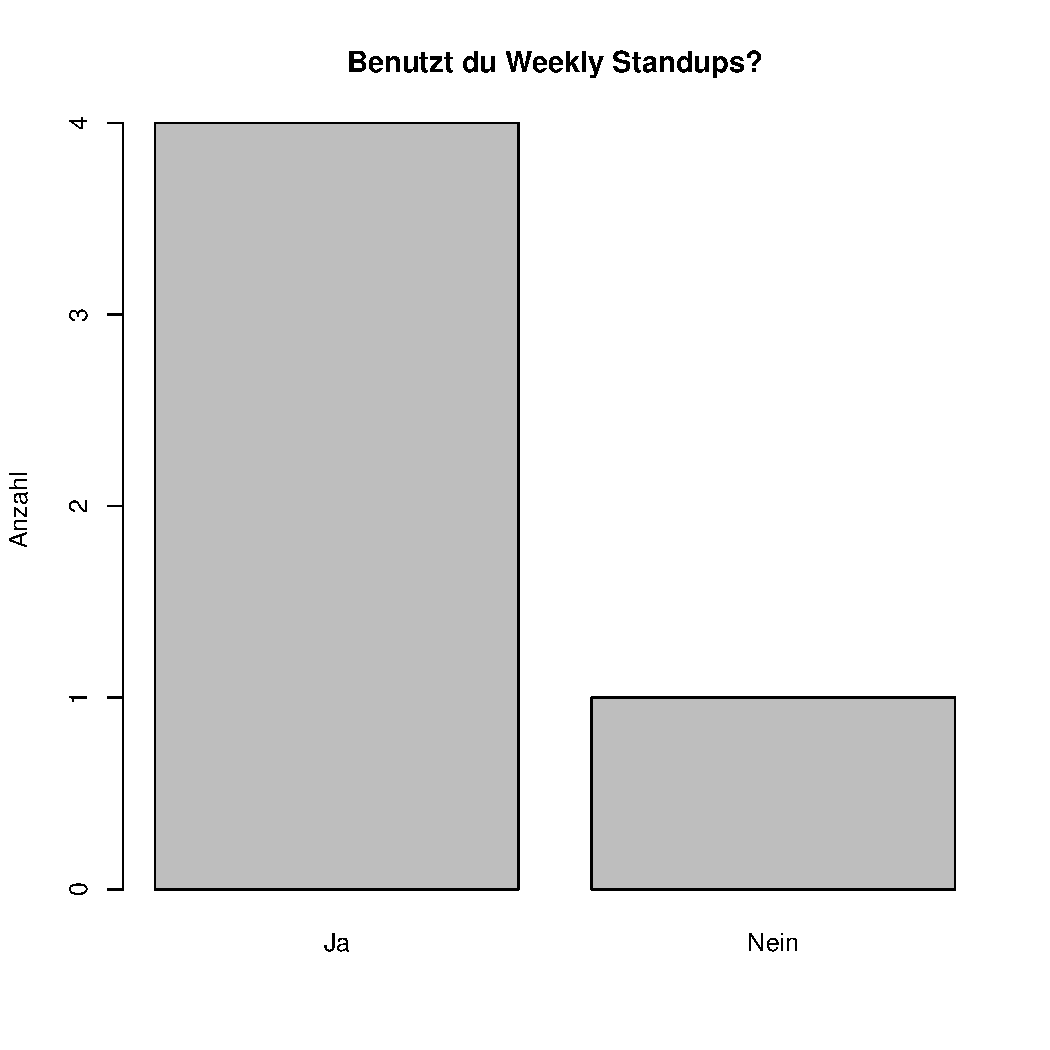
\includegraphics[width=0.40\textwidth]{q1.pdf}
    \caption{Verwendung von Weekly Standups unter den Befragten}
	\label{fig:q1}
\end{figure}
\textbf{Ergebnis:} Den meisten ist das Weekly Standup geläufig.
\subsection{Frage 2: Welcher Nutzergruppe gehörst du an?}
Damit wir sicherstellen das wir mit unseren Personas richtig liegen haben wir gefragt in welche Gruppe sich die befragten einordnen würden.
\begin{figure}[H]
	\centering
	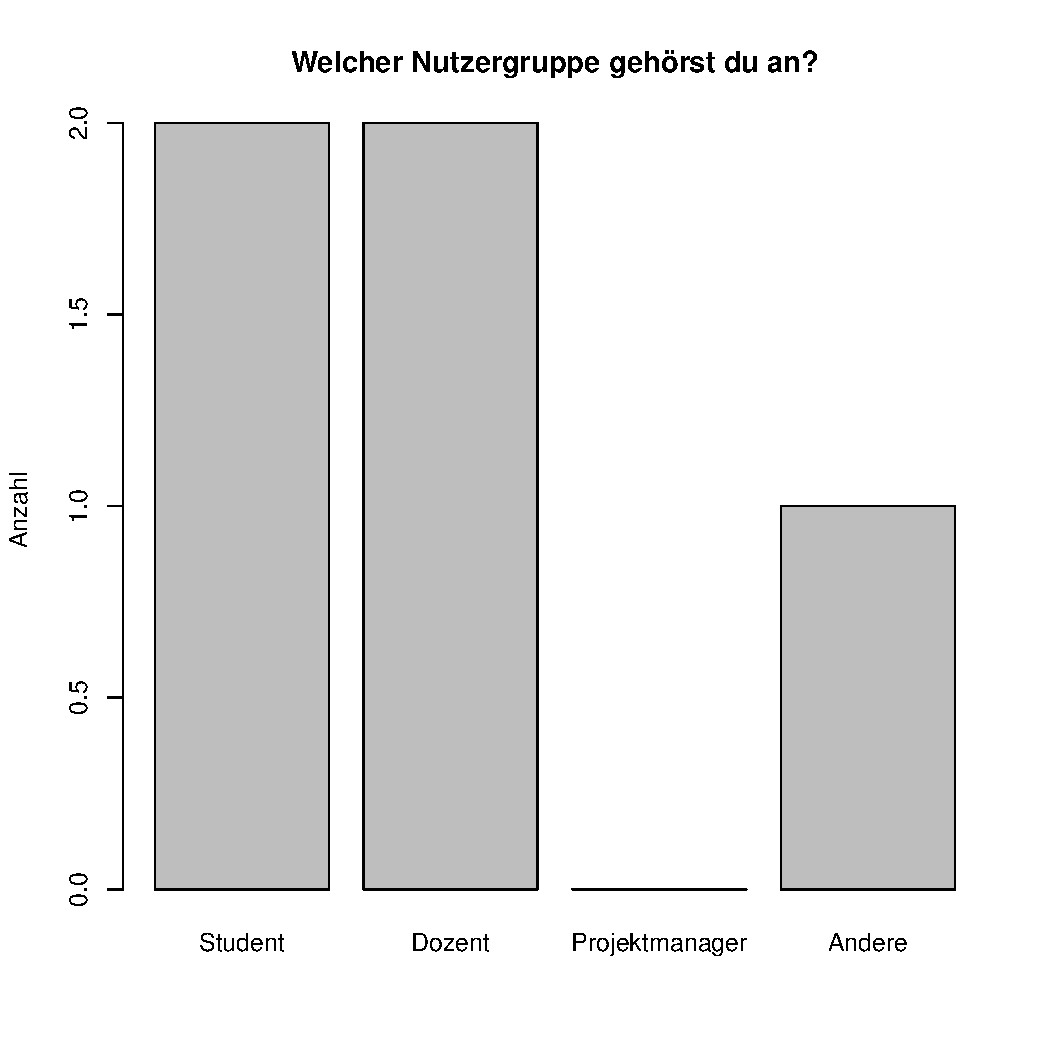
\includegraphics[width=0.40\textwidth]{q2.pdf}
    \caption{Nutzergruppe der Befragten}
	\label{fig:q2}
\end{figure}
\textbf{Ergebnis:} Unsere Personas sind für die Befragten zutreffend.
\subsection{Frage 3: Welche Projektarten führst du aus?}
Hiermit möchten wir erfahren mit welcher Art von Projekten die potenziellen Nutzer schon Kontakt hatten. 
\begin{figure}[H]
	\centering
	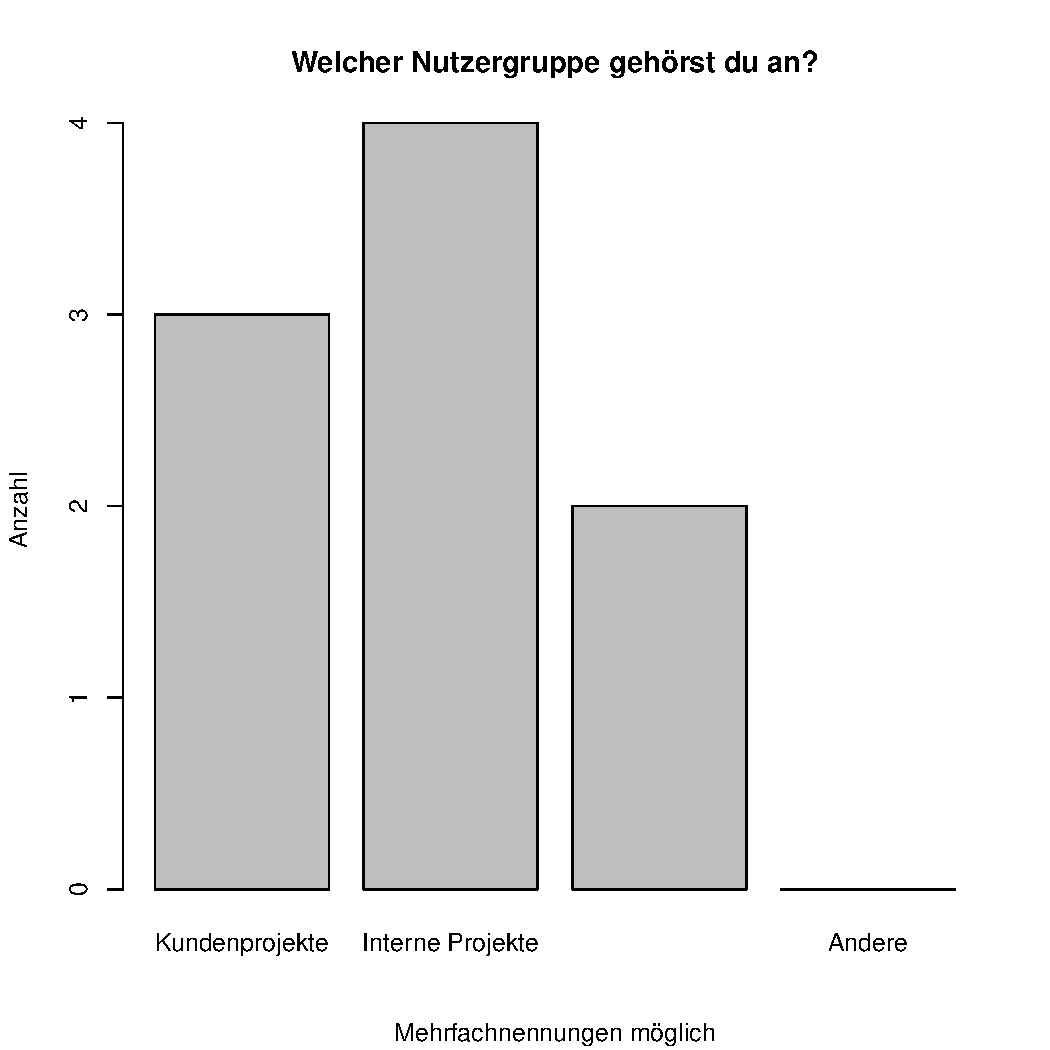
\includegraphics[width=0.40\textwidth]{q3.pdf}
    \caption{Projektarten der Befragten}
	\label{fig:q3}
\end{figure}
\textbf{Ergebnis:} Hier ergibt sich das sich die befragten hauptsächlich mit internen oder Kundenprojekten beschäftigen. Das Weekly standup soll nach die Kommunikation in Projekten unterstützen, was gerade bei Projekten mit Kunden wichtig ist.
\subsection{Frage 4: Wie alt bist du?} 
\begin{figure}[H]
	\centering
	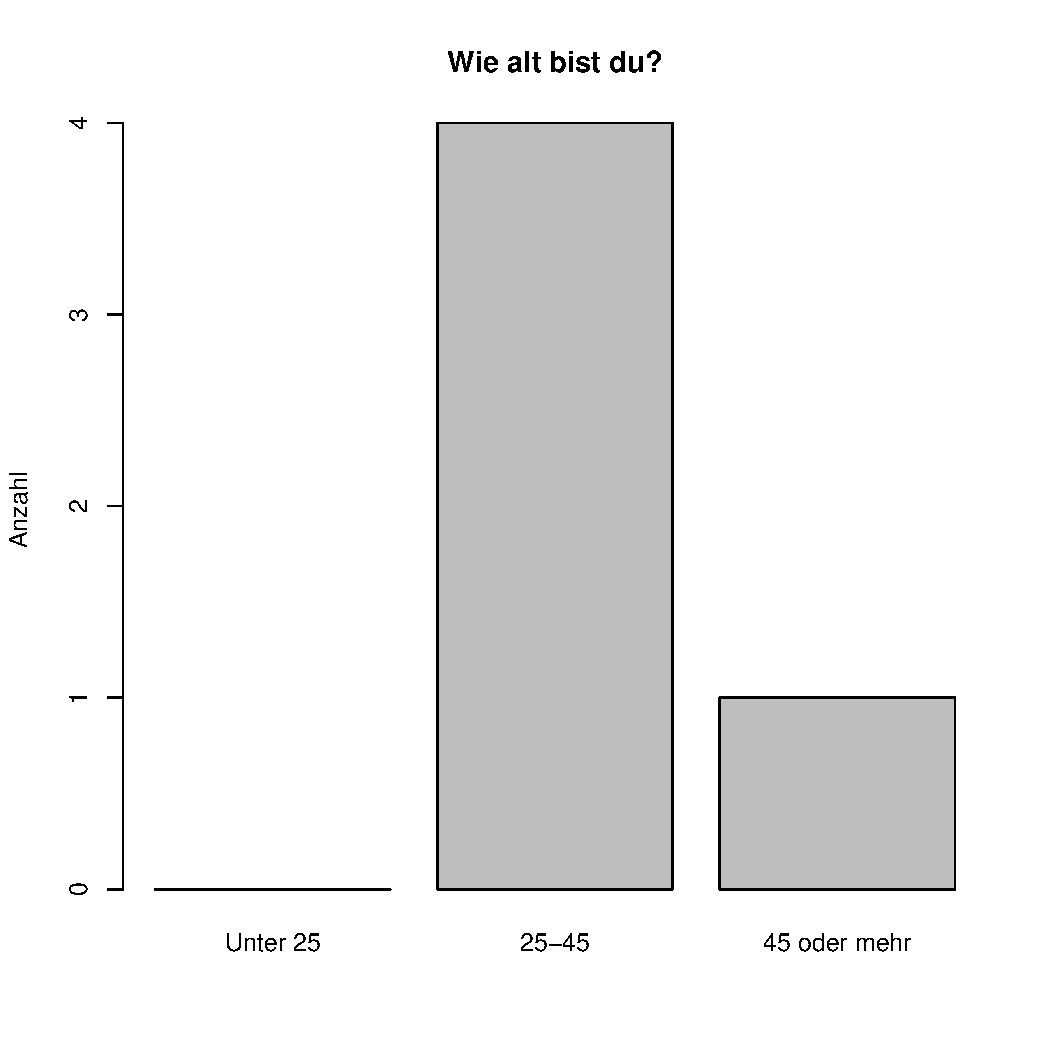
\includegraphics[width=0.40\textwidth]{q4.pdf}
    \caption{Alter der Befragten}
	\label{fig:q4}
\end{figure}     
\subsection{Frage 5: Wie viel Zeit verbringst du Wöchentlich in Standup Meetings?}
Eines unsere Ziele soll sein die Zeit welche Nutzer in meetings verbringen zu Reduzieren. Daher wollen wir wissen wiviel Zeit Nutzer in Weekly Standups im schnitt verbringen.
\begin{figure}[H]
	\centering
	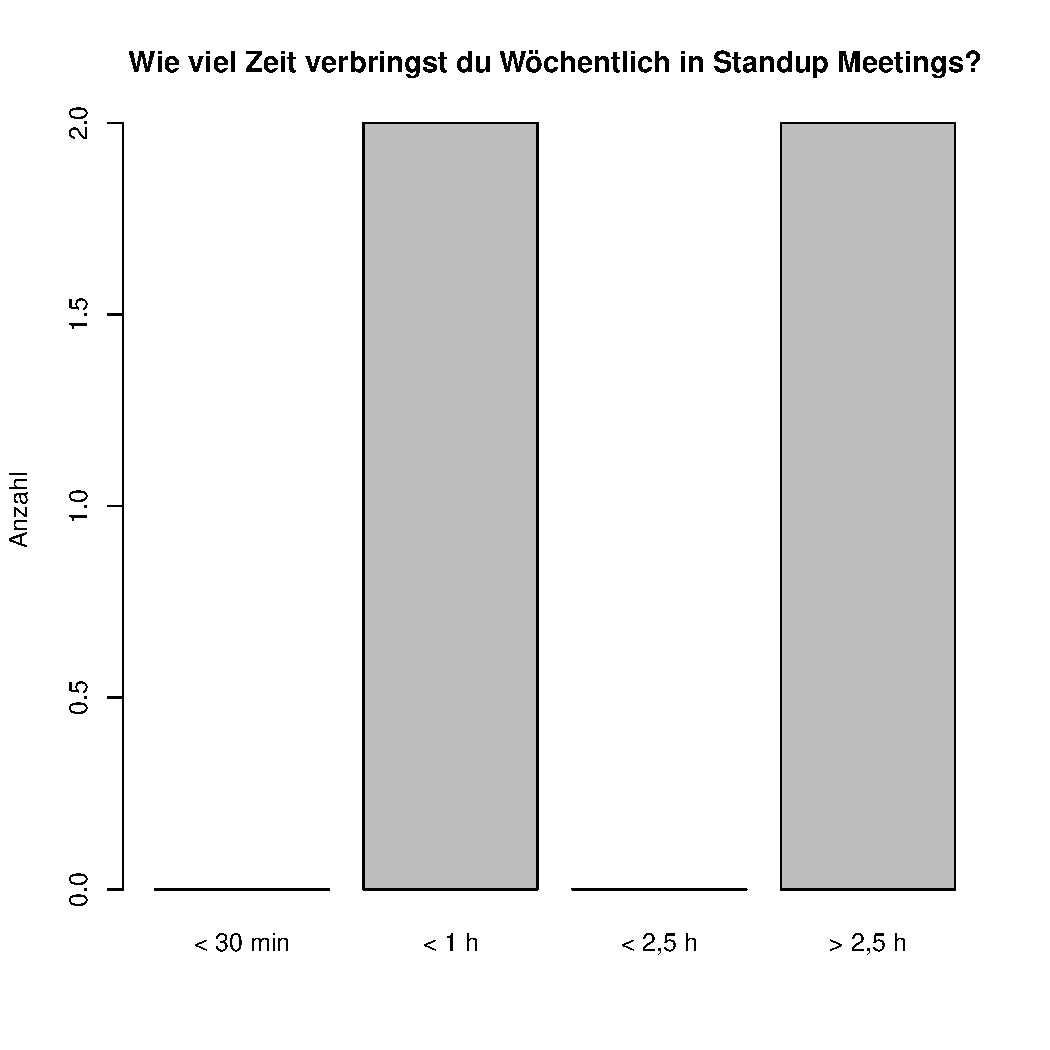
\includegraphics[width=0.40\textwidth]{q5.pdf}
    \caption{Zeit welche die Befragten in Statusmeetings verbringen}
	\label{fig:q5}
\end{figure}
\textbf{Ergebnis:} Unsere angepeilte Bearbeitungszeit von < 10 Minuten würde für alle Nutzer eine deutliche Reduktion von Zeitaufwänden darstellen
\subsection{Frage 6: Wie hilfreich findest du Weekly Standups?}

\begin{figure}[H]
	\centering
	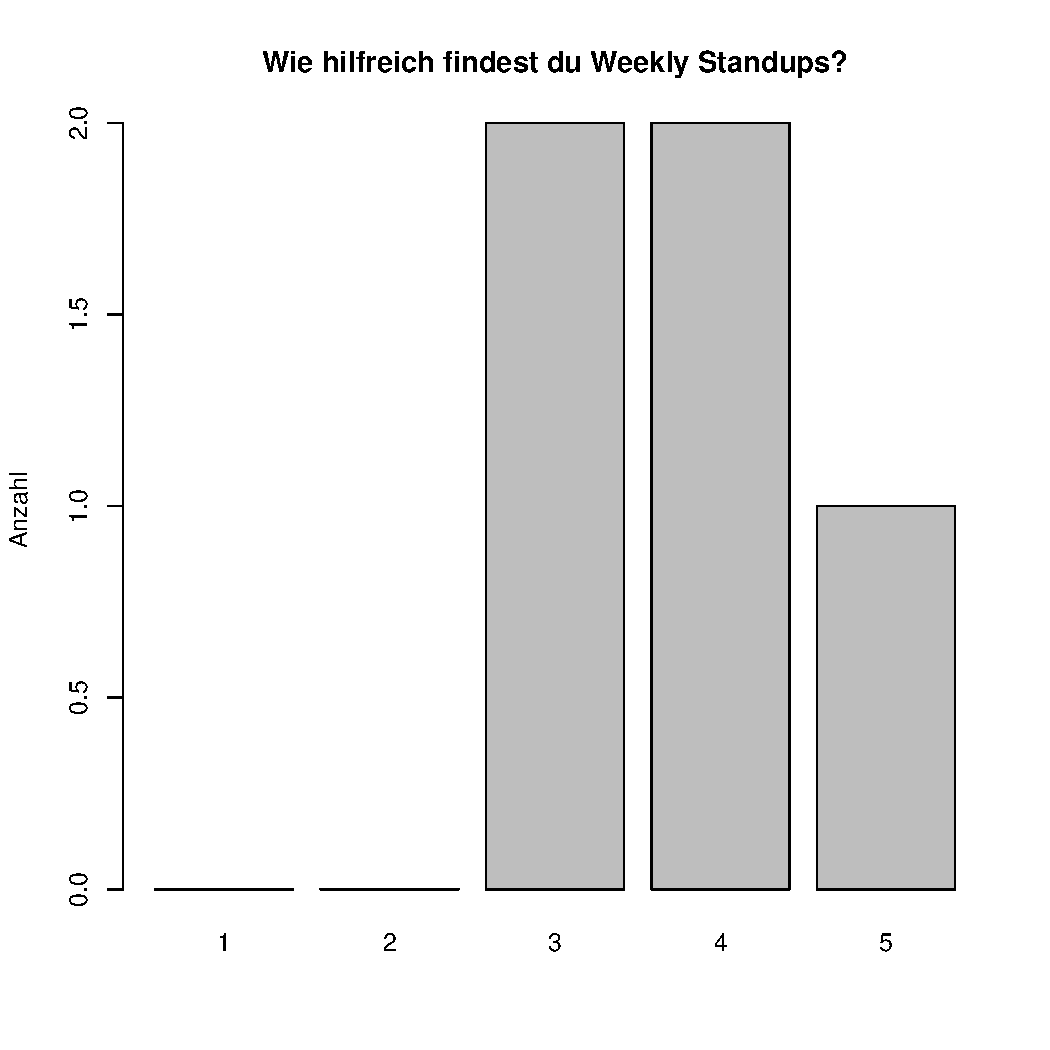
\includegraphics[width=0.40\textwidth]{q6.pdf}
    \caption{Gefühlter Nutzen eines Weekly Standups}
	\label{fig:q6}
\end{figure}  
\subsection{Frage 7: Wie arbeitest du zur Zeit?}
Aufgrund der aktuellen Lage erschien es uns wichtig herauszufinden ob die Befragten eher vor Ort oder Remote arbeiten.
\begin{figure}[H]
	\centering
	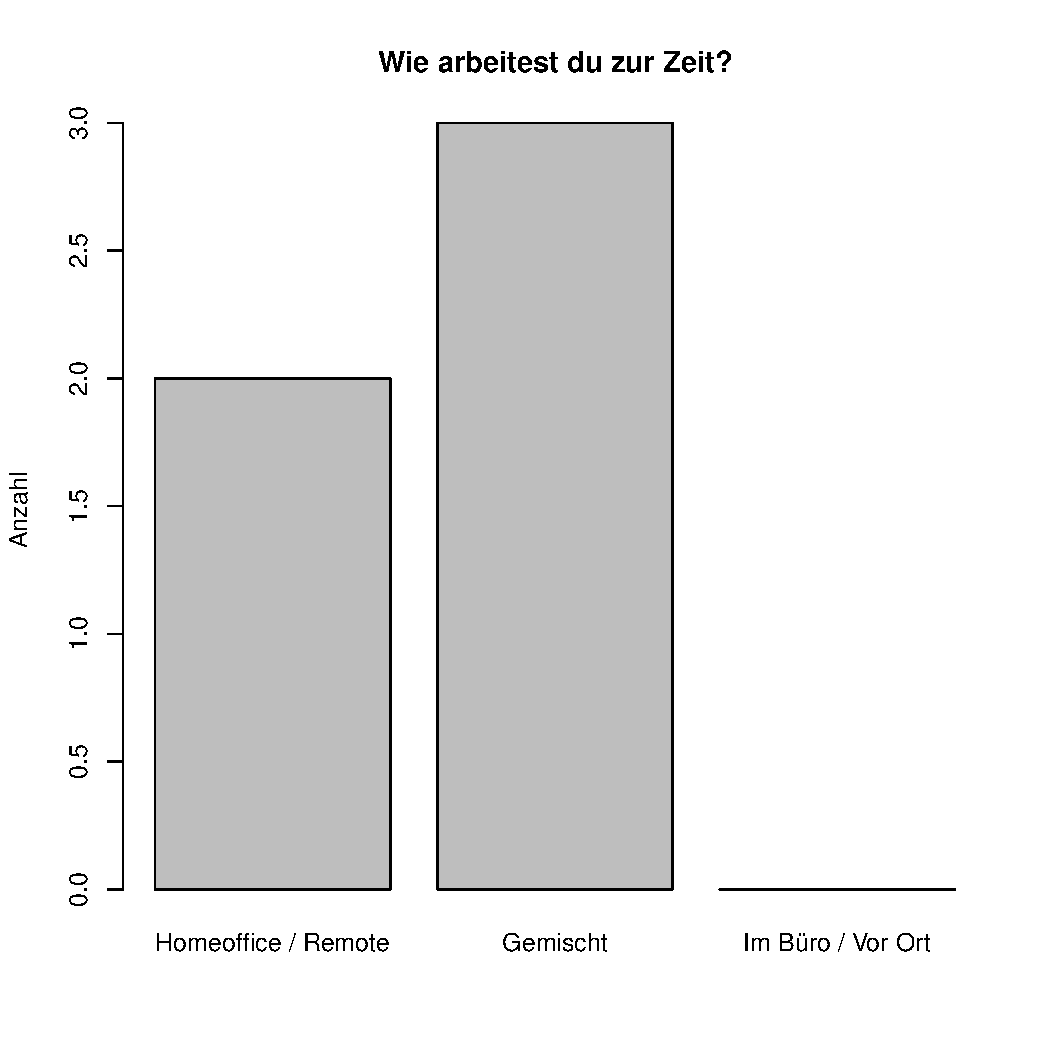
\includegraphics[width=0.40\textwidth]{q7.pdf}
    \caption{Arbeitsumfeld der Befragten}
	\label{fig:q7}
\end{figure}  
\textbf{Ergebnis:} Alle Befragten arbeiten zumindest teilweise Remote, dies würde die Verwendung eines Onlinetools nahelegen.
\subsection{Frage 8: Wie bewertest du folgende Features?}
Um eine Priorisierung unserer geplanten Featuers vornehmen zu können haben wir die Nutzer gebeten bestimmte Funktionalitäten auf ihren potenziellen nutzen hin zu bewerten. 
\subsubsection{Frage 8.1: Erinnerung}
\begin{figure}[H]
	\centering
	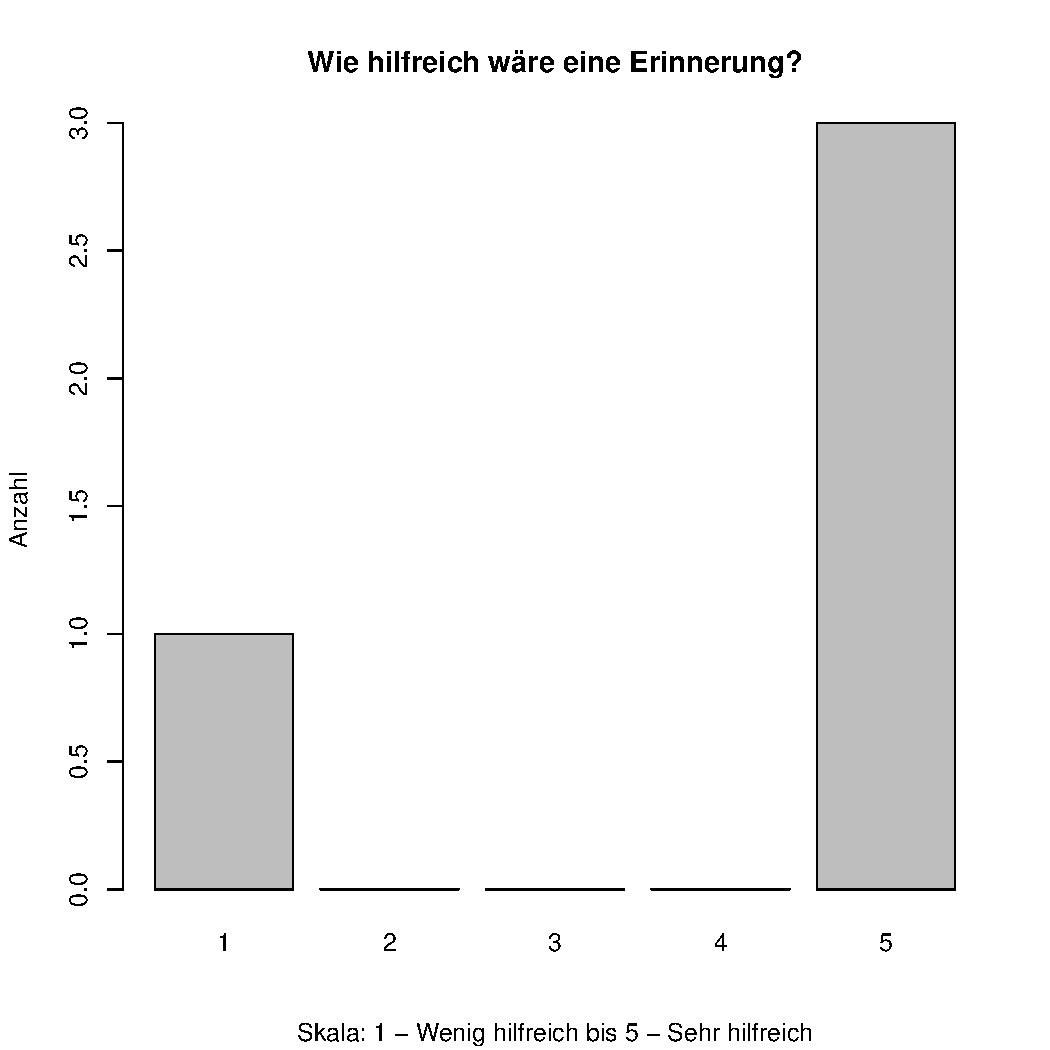
\includegraphics[width=0.40\textwidth]{q8-1.pdf}
    \caption{Nützlichkeit einer Erinnerung}
	\label{fig:q81}
\end{figure} 
\textbf{Ergebnis:} Die meisten Nutzer würden sich über eine Erinnerung (bei Nichtteilnahme) wünschen.
\subsubsection{Frage 8.2: Timeline}
\begin{figure}[H]
	\centering
	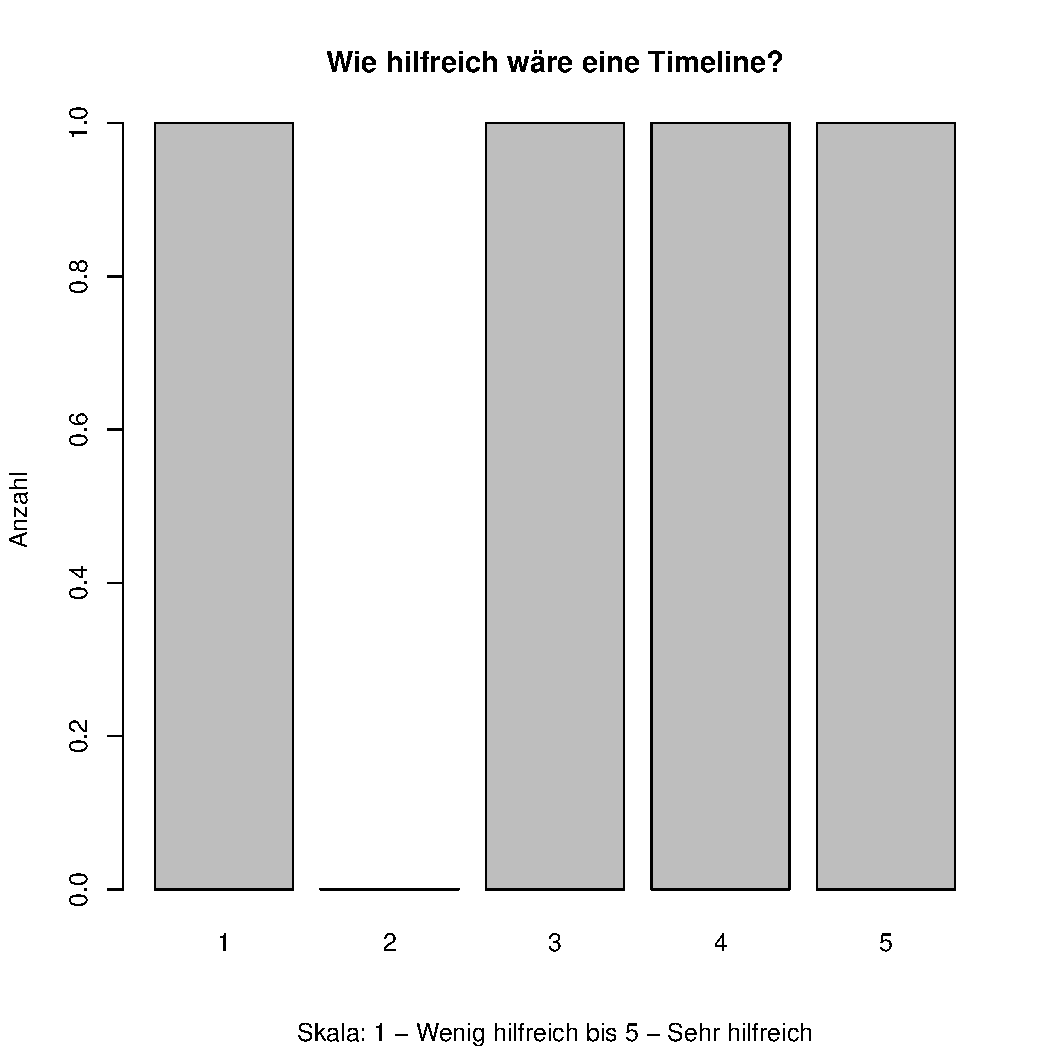
\includegraphics[width=0.40\textwidth]{q8-2.pdf}
    \caption{Nützlichkeit einer Timeline}
	\label{fig:q82}
\end{figure} 
\textbf{Ergebnis:} Das Thema Timeline kann mit nachgeordneter Priorität behandelt werden, hier ergab sich keine eindeutige Präferenz.
\subsubsection{Frage 8.3: Suche}
\begin{figure}[H]
	\centering
	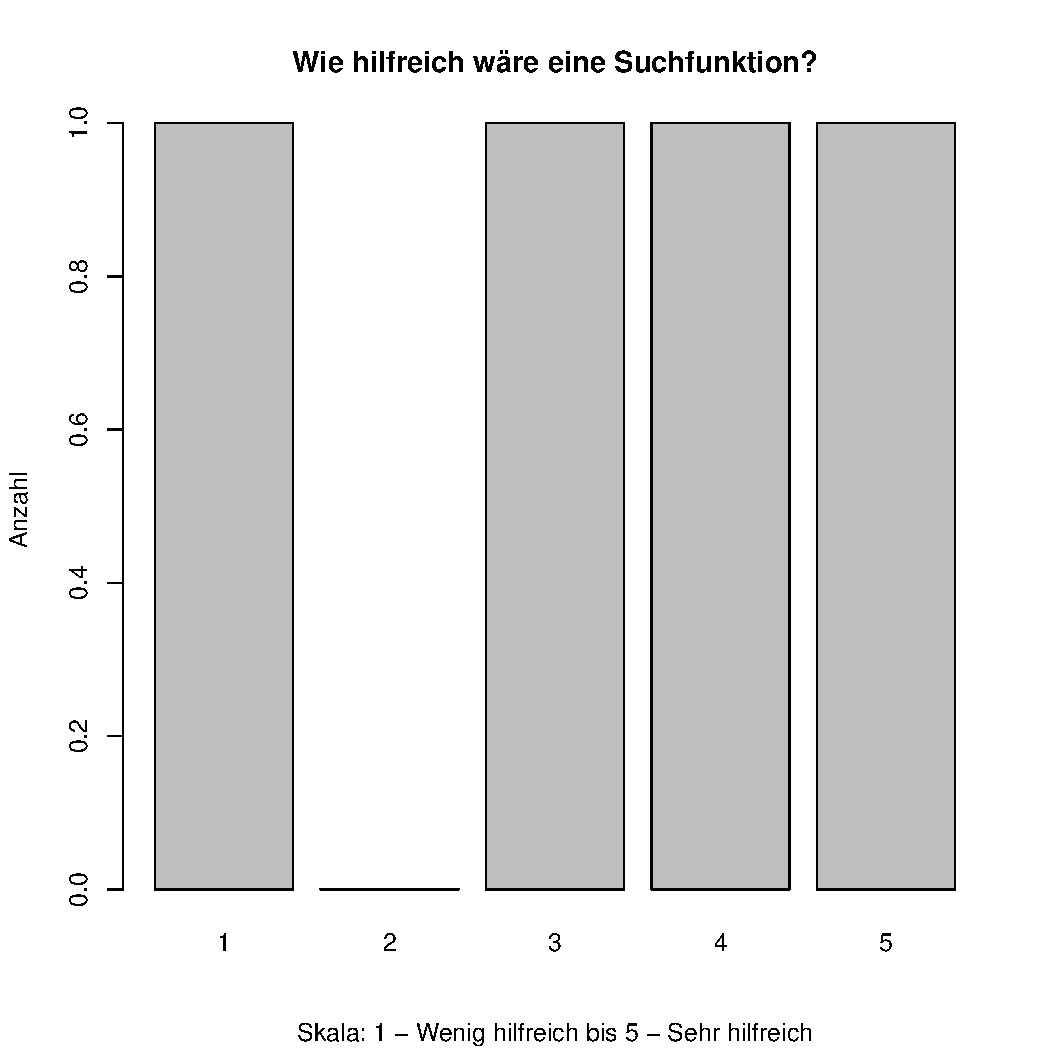
\includegraphics[width=0.40\textwidth]{q8-3.pdf}
    \caption{Nützlichkeit einer Suche}
	\label{fig:q83}
\end{figure} 
\textbf{Ergebnis:} Das Thema Suche kann mit nachgeordneter Priorität behandelt werden, hier ergab sich keine eindeutige Präferenz.

\subsubsection{Frage 8.4: Markieren}
\begin{figure}[H]
	\centering
	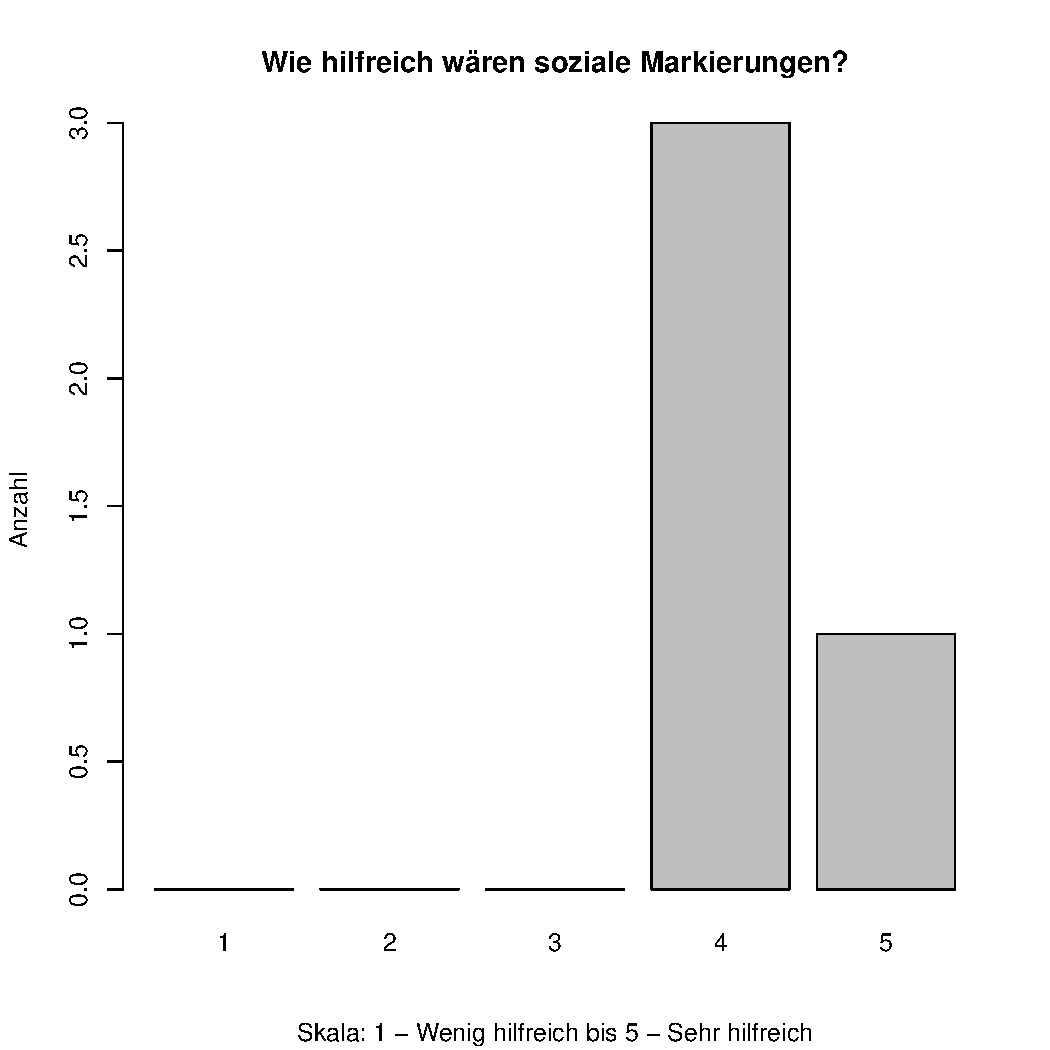
\includegraphics[width=0.40\textwidth]{q8-4.pdf}
    \caption{Nützlichkeit von Markierungen}
	\label{fig:q84}
\end{figure} 
\textbf{Ergebnis:} Das markieren von Einträgen für ein niederschwelliges Feedback scheint den meisten Nutzern als hilfreich.
\subsubsection{Frage 8.5: Vorgegebene Eingabefelder}
\begin{figure}[H]
	\centering
	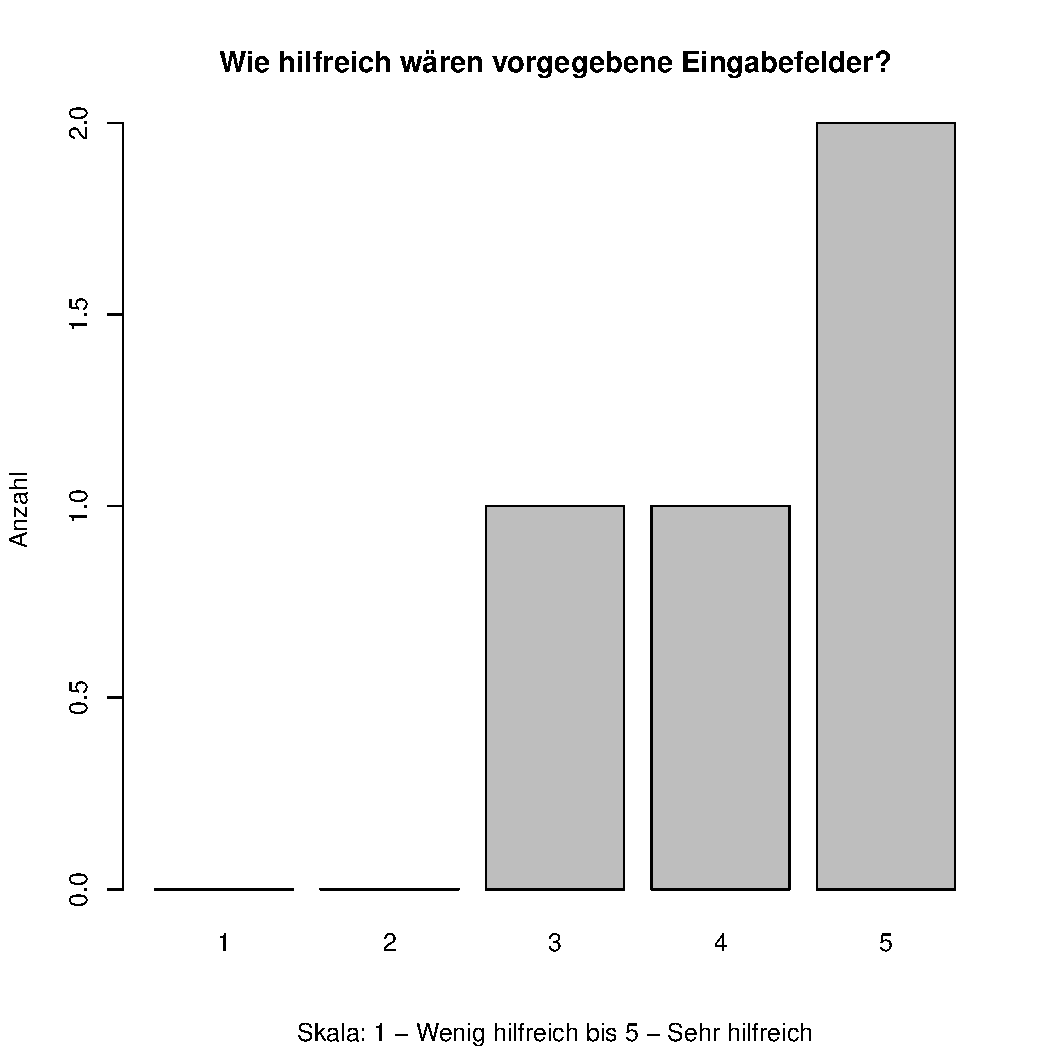
\includegraphics[width=0.40\textwidth]{q8-5.pdf}
    \caption{Nützlichkeit von Vorgaben}
	\label{fig:q85}
\end{figure}
\textbf{Ergebnis:} Vorgaben für die Eingabefelder, gerade für unerfahrene Nutzer, werden als potenziell hilfreich eingestuft, jedoch nicht so nachdrücklich wie andere Features.
\subsection{Frage 9: Was ist dein bevorzugter Zeitpunkt für ein Weekly Standup?}
Für das Verschicken der Erinnerung wollten wissen wann die Nutzer normalerweise ihr Standup bevorzugen.
\begin{figure}[H]
	\centering
	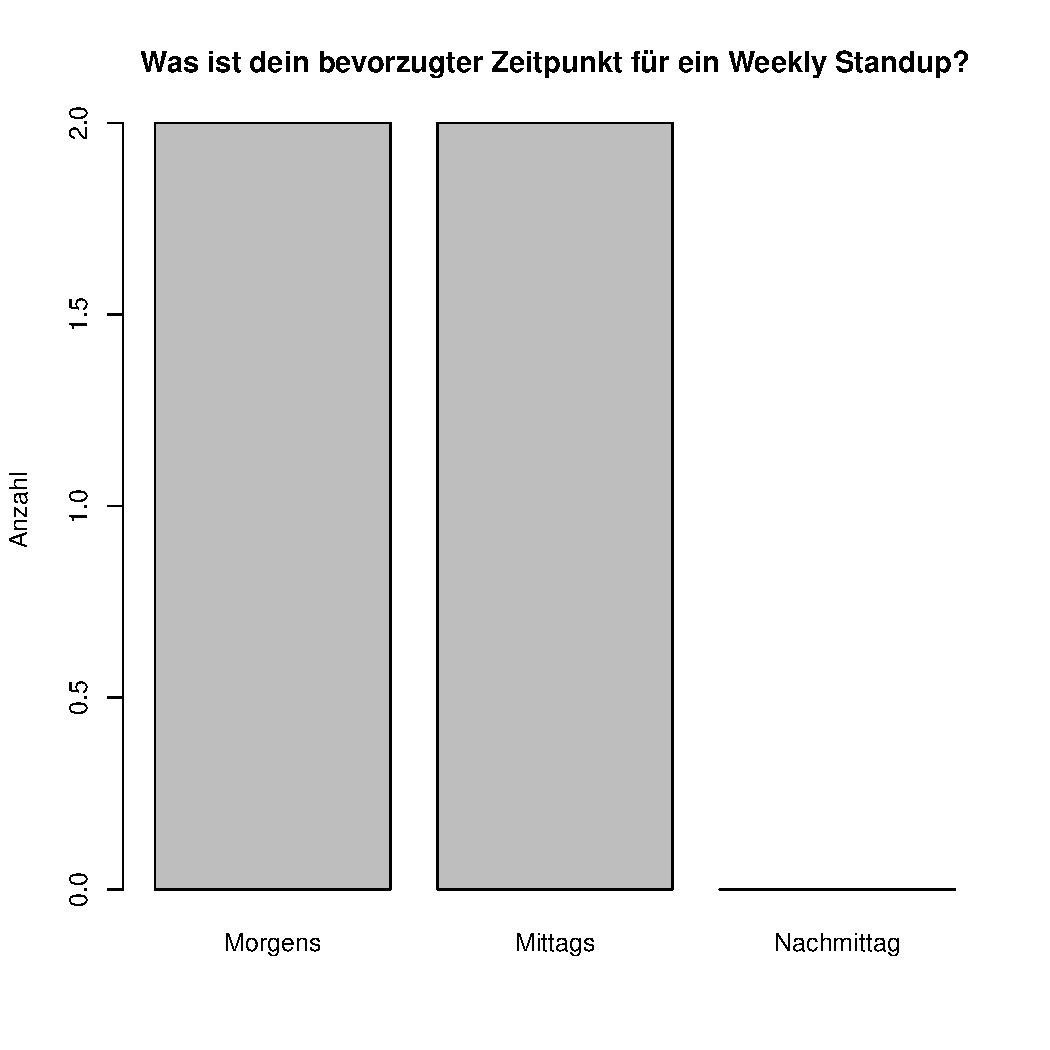
\includegraphics[width=0.40\textwidth]{q9.pdf}
    \caption{Idealer Zeitpunkt für ein Weekly Standup}
	\label{fig:q9}
\end{figure}  
\subsection{Frage 10: Welche Form eines Weekly Standups würdest du bevorzugen?}
Um die Bereitschaft ein rein schriftliches Weekly Standup durchzuführen abzuschätzen wollten wir wissen welche Art von meetings die Nutzer bevorzugen.
\begin{figure}[H]
	\centering
	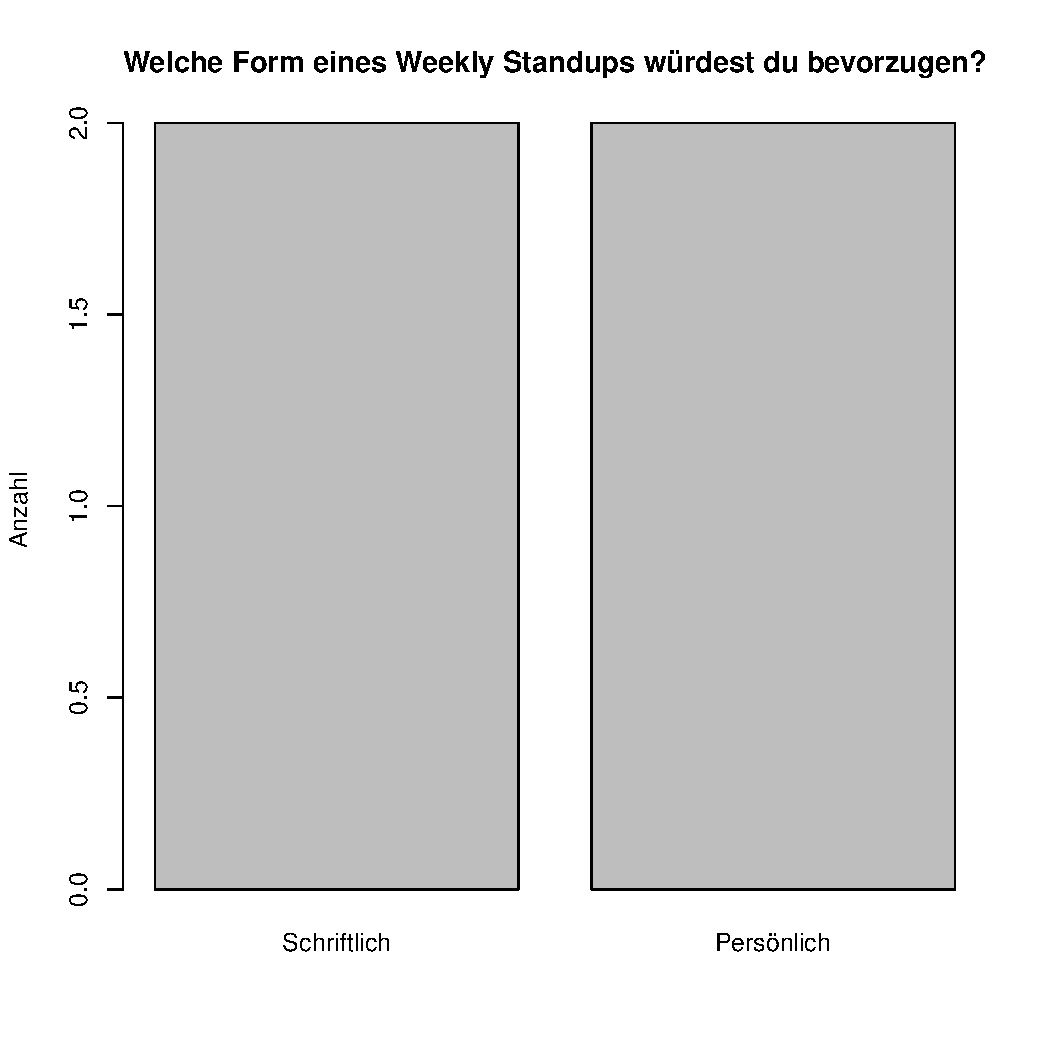
\includegraphics[width=0.40\textwidth]{q10.pdf}
    \caption{Bevorzugte form des Weekly Standups}
	\label{fig:q10}
\end{figure} 
\subsection{Frage 11: Würdest du einen Chatbot als hilfreich empfinden, welcher dir Informationen wie Deployment, Status, Logereignisse im Meeting mitteilt?}
Diese Frage zielt auf ein ursprünglich geplantes Feature ab.
\begin{figure}[H]
	\centering
	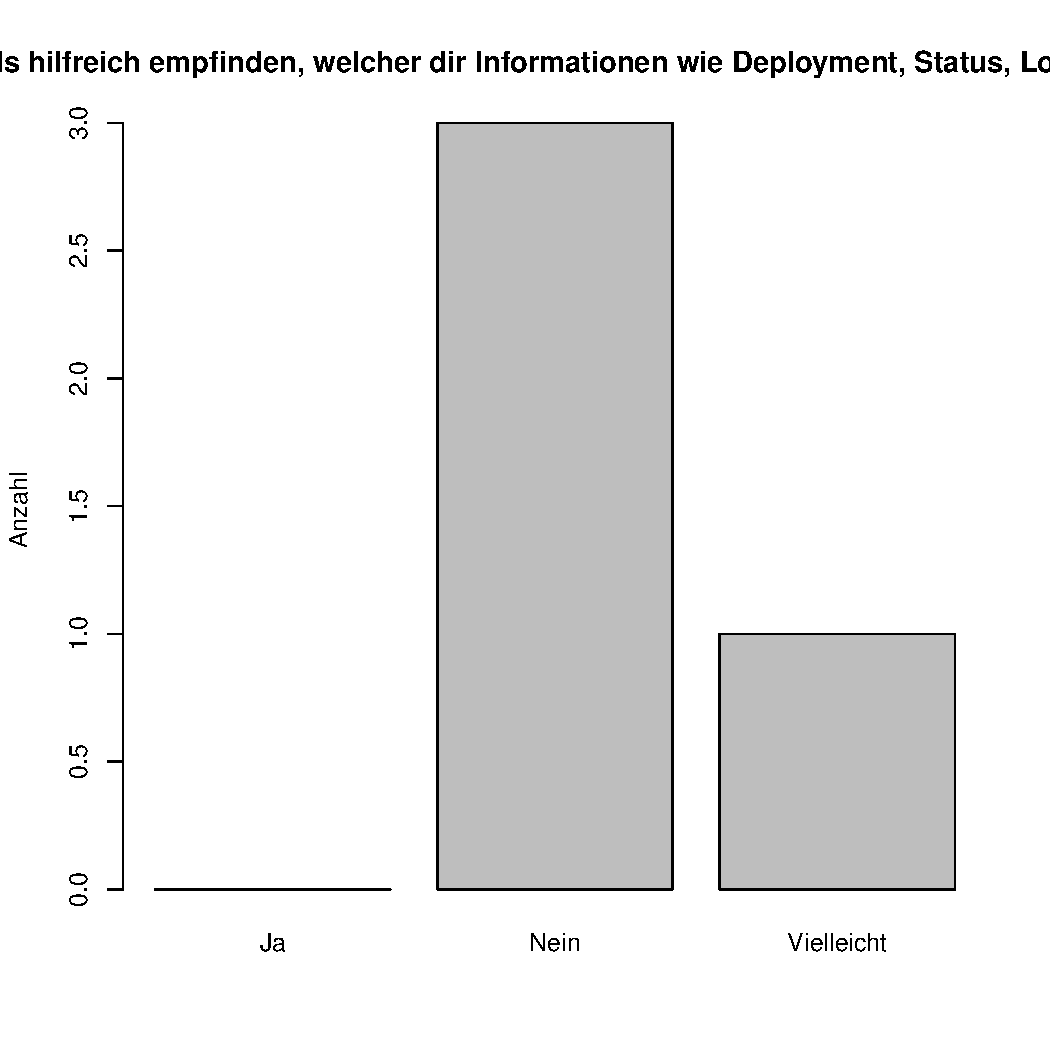
\includegraphics[width=0.40\textwidth]{q11.pdf}
    \caption{Meinung zu einem Chatbot}
	\label{fig:q11}
\end{figure} 
\textbf{Ergebnis:} Eine Integration von Chatbots scheint den Nutzern im Kontext des Weekly Standups nicht wichtig zu sein.

\subsection{Frage 12: Welche Informationen wären für dich als Projektmanager in einem Weekly Standup wichtig?}
Diese Frage wurde als Freitextaufgabe gestellt. Zwei der befragten haben sich dazu geäußert und folgende Informationen als wünschenswert zu erheben herausgestellt:
\begin{itemize}
\item Verknüpfung zu Aufgaben -> Überblick in Bezug auf den Plan
\item Muss ich als Dozent / PM intervenieren / Resourcen / Unterstützung / Hilfestellungen bereitstellen? 
\item Wer macht / wie viel mit? 
\item Gibt es Abwesenheiten?
\end{itemize}

\subsection{Frage 13: Wenn du bereits Weekly Standups gemacht hast, welche Tools hast du dafür benutzt?}
Bei dieser Frage handelte es sich wiederum um eine Freitext eingabe. die am häufigsten genannten Tools waren hierbei:
\begin{itemize}
    \item Jira (3x)
    \item Teams (3x)
    \item Miro
    \item Jitsi
\end{itemize}
Aber auch dinge wie Azure Devops oder digitale/smarte Whiteboards wurden genannt.

\subsection{Frage 14: Wie wichtig wäre dir eine Zeitbegrenzung des Meetings?}
\begin{figure}[H]
	\centering
	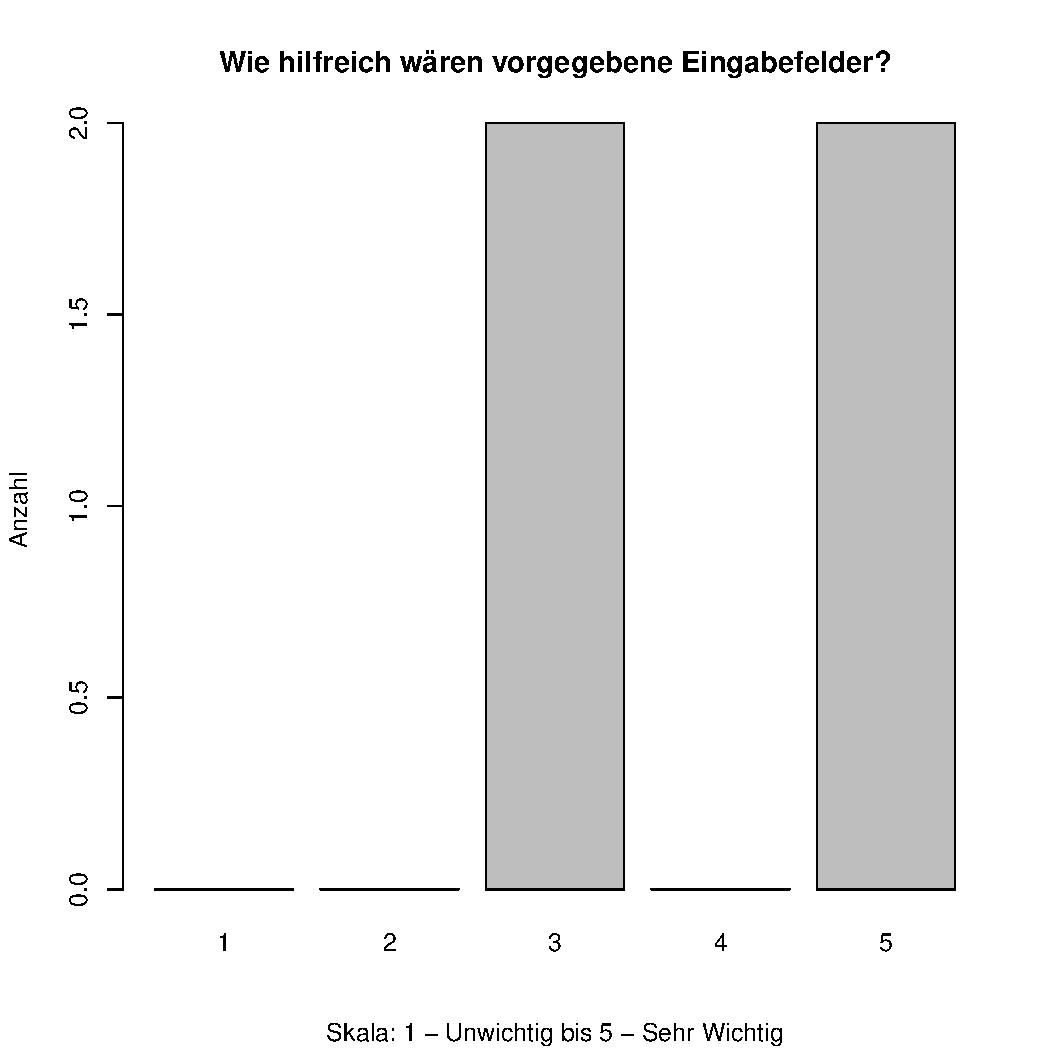
\includegraphics[width=0.40\textwidth]{q14.pdf}
    \caption{Wunsch nach Zeitbegrenzung}
	\label{fig:q14}
\end{figure} 
\section{Methodik}



